% !TEX root = ../entropy.tex

\section{Spending profiles predict emergency savings}%
\label{sec:results}

Table~\ref{tab:reg_has_inflows_main} shows the effect of entropy on the
probability of building emergency savings in a given month. Columns (1)-(3)
show results for unsmoothed entropy based on 9 categories, 48 categories, and
merchant names, respectively. Columns (4)-(6) results for smoothed entropy
based on the same variables. All models include user and year-month fixed
effects, and standard errors are clustered at the user-level. 95\% confidence
intervals are shown in brakets.


\begin{table}[htbp]
   \centering
   \tiny
   \begin{threeparttable}[b]
      \caption{\label{tab:reg_has_inflows_main} Effect of entropy on P(transfer into savings accounts)}
      \begin{tabular}{lcccccc}
         \tabularnewline \midrule \midrule
         Model:                     & (1)             & (2)             & (3)             & (4)              & (5)              & (6)\\  
         \midrule
         \emph{Variables}\\
         Entropy (9 cats)           & 0.016$^{***}$   &                 &                 &                  &                  &   \\   
                                    & [0.013; 0.019]  &                 &                 &                  &                  &   \\   
         Entropy (48 cats)          &                 & 0.029$^{***}$   &                 &                  &                  &   \\   
                                    &                 & [0.025; 0.033]  &                 &                  &                  &   \\   
         Entropy (merchant)         &                 &                 & 0.032$^{***}$   &                  &                  &   \\   
                                    &                 &                 & [0.029; 0.036]  &                  &                  &   \\   
         Entropy (9 cats, smooth)   &                 &                 &                 & -0.008$^{***}$   &                  &   \\   
                                    &                 &                 &                 & [-0.010; -0.006] &                  &   \\   
         Entropy (48 cats, smooth)  &                 &                 &                 &                  & -0.023$^{***}$   &   \\   
                                    &                 &                 &                 &                  & [-0.025; -0.020] &   \\   
         Entropy (merchant, smooth) &                 &                 &                 &                  &                  & -0.019$^{***}$\\   
                                    &                 &                 &                 &                  &                  & [-0.021; -0.016]\\   
         Month spend                & 0.009$^{***}$   & 0.009$^{***}$   & 0.008$^{***}$   & 0.009$^{***}$    & 0.008$^{***}$    & 0.007$^{***}$\\   
                                    & [0.009; 0.010]  & [0.008; 0.009]  & [0.008; 0.009]  & [0.009; 0.010]   & [0.007; 0.009]   & [0.007; 0.008]\\   
         Month income               & 0.012$^{***}$   & 0.012$^{***}$   & 0.012$^{***}$   & 0.012$^{***}$    & 0.011$^{***}$    & 0.011$^{***}$\\   
                                    & [0.011; 0.013]  & [0.011; 0.013]  & [0.011; 0.013]  & [0.011; 0.013]   & [0.011; 0.012]   & [0.010; 0.012]\\   
         Has income in month        & 0.086$^{***}$   & 0.084$^{***}$   & 0.083$^{***}$   & 0.087$^{***}$    & 0.085$^{***}$    & 0.086$^{***}$\\   
                                    & [0.077; 0.094]  & [0.075; 0.092]  & [0.074; 0.091]  & [0.079; 0.096]   & [0.076; 0.093]   & [0.078; 0.095]\\   
         Income variability         & 0.001$^{*}$     & 0.001$^{*}$     & 0.001$^{*}$     & 0.001$^{*}$      & 0.001$^{*}$      & 0.000\\   
                                    & [-0.000; 0.001] & [-0.000; 0.001] & [-0.000; 0.001] & [-0.000; 0.001]  & [-0.000; 0.001]  & [-0.000; 0.001]\\   
         \midrule
         \emph{Fixed-effects}\\
         User                       & Yes             & Yes             & Yes             & Yes              & Yes              & Yes\\  
         Year-month                 & Yes             & Yes             & Yes             & Yes              & Yes              & Yes\\  
         \midrule
         \emph{Fit statistics}\\
         Observations               & 1,043,727       & 1,043,727       & 1,043,416       & 1,043,727        & 1,043,727        & 1,043,416\\  
         R$^2$                      & 0.45368         & 0.45395         & 0.45410         & 0.45363          & 0.45415          & 0.45410\\  
         Within R$^2$               & 0.00719         & 0.00768         & 0.00807         & 0.00709          & 0.00805          & 0.00808\\  
         \midrule \midrule
         \multicolumn{7}{l}{\emph{Clustered (User) co-variance matrix, 95\% confidence intervals in brackets}}\\
         \multicolumn{7}{l}{\emph{Signif. Codes: ***: 0.01, **: 0.05, *: 0.1}}\\
      \end{tabular}
   \end{threeparttable}
\end{table}




Results for unsmoothed entropy suggest that a one unit increase in entropy is
associated with an increase in the probability of a user making at least one
transfer into their savings accounts of between 1.5 and 2.7 percentage points
-- an effect up to two times larger than that of a \pounds1000 increase in
monthly income. Conversely, the effect for unsmooth entropy is smaller in
magnitude but runs in the reverse direction: a one-unit increase in the
smoothed entropy score is associated with a reduction in the probability of
transferring money into savings account of between 0.4 and 1.6 percentage
points -- an effect that, in absolute magnitude, is about equal to that of a
\pounds1000 increase in monthly income.

As discussed in Section~\ref{sub:estimation}, these results are not a results
of reverse causality. While we might think that making a savings transactions
might change some or all of the components of entropy discussed in
Section~\ref{sub:spending_profiles} -- the number of unique spending categories
with positive frequency count, the standard deviation of these counts, and the
total number of spend transactions -- and thus change entropy, this is not the
case because of the way we define entropy and savings, and the way spending
transactions are categorised. We define entropy based on all current account
debits that are identified as spends, while we define savings transactions as
the sum of all savings accounts credits. If a user transfers money from their
current account to their savings account, this will be identified as a savings
transaction, but be identified as a transfer on their current account and thus
not considered when calculating their entropy score.

Overall, the effect of entropy in spending profiles is statistically and
economically significant, and robust across different definitions. In other
words, the scores seem to pick up a feature of the spending distribution that
is predictive of savings behaviour.

Two questions remain: first, does entropy capture an element of the spending
distributions that is different from what is captured by its three main
components? Second, why does smoothing entropy scores flip the direction of the
effec? We will address these in turn.


\subsection{Is entropy more than the sum of its parts?}%
\label{sub:is_entropy_more_than_the_sum_of_its_parts_}

In Section~\ref{sub:spending_profiles} we show that we can think of both
unsmoothed and smoothed entropy as a fundtion of three simple components: the
number of unqiue spending categories with a positive frequency count, the
standard deviation of those counts, and the number of spending transactions.
Here we want to test whether entropy remains predictive of savings behaviour
once we control for these components.


\begin{table}[htbp]
   \centering
   \tiny
   \begin{threeparttable}[b]
      \caption{\label{tab:reg_has_inflows_comp} Controlling for entropy components}
      \begin{tabular}{lcccc}
         \tabularnewline \midrule \midrule
         Model:                    & (1)             & (2)             & (3)              & (4)\\  
         \midrule
         \emph{Variables}\\
         Entropy (48 cats)         & 0.029$^{***}$   & 0.013$^{***}$   &                  &   \\   
                                   & [0.025; 0.033]  & [0.006; 0.021]  &                  &   \\   
         Entropy (48 cats, smooth) &                 &                 & -0.023$^{***}$   & -0.028$^{***}$\\   
                                   &                 &                 & [-0.025; -0.020] & [-0.034; -0.022]\\   
         Unique categories         &                 & 0.004$^{***}$   &                  & 0.004$^{***}$\\   
                                   &                 & [0.003; 0.005]  &                  & [0.004; 0.005]\\   
         Category counts std.      &                 & 0.002           &                  & -0.015$^{***}$\\   
                                   &                 & [-0.001; 0.006] &                  & [-0.018; -0.011]\\   
         Number of spend txns      &                 & 0.000$^{***}$   &                  & 0.001$^{***}$\\   
                                   &                 & [0.000; 0.001]  &                  & [0.001; 0.001]\\   
         Month spend               & 0.009$^{***}$   & 0.005$^{***}$   & 0.008$^{***}$    & 0.005$^{***}$\\   
                                   & [0.008; 0.009]  & [0.004; 0.006]  & [0.007; 0.009]   & [0.005; 0.006]\\   
         Month income              & 0.012$^{***}$   & 0.011$^{***}$   & 0.011$^{***}$    & 0.011$^{***}$\\   
                                   & [0.011; 0.013]  & [0.010; 0.012]  & [0.011; 0.012]   & [0.010; 0.012]\\   
         Has income in month       & 0.084$^{***}$   & 0.079$^{***}$   & 0.085$^{***}$    & 0.078$^{***}$\\   
                                   & [0.075; 0.092]  & [0.070; 0.087]  & [0.076; 0.093]   & [0.070; 0.087]\\   
         Income variability        & 0.001$^{*}$     & 0.000           & 0.001$^{*}$      & 0.000\\   
                                   & [-0.000; 0.001] & [-0.000; 0.001] & [-0.000; 0.001]  & [-0.000; 0.001]\\   
         \midrule
         \emph{Fixed-effects}\\
         User                      & Yes             & Yes             & Yes              & Yes\\  
         Year-month                & Yes             & Yes             & Yes              & Yes\\  
         \midrule
         \emph{Fit statistics}\\
         Observations              & 1,043,727       & 1,043,727       & 1,043,727        & 1,043,727\\  
         R$^2$                     & 0.45395         & 0.45498         & 0.45415          & 0.45515\\  
         Within R$^2$              & 0.00768         & 0.00956         & 0.00805          & 0.00986\\  
         \midrule \midrule
         \multicolumn{5}{l}{\emph{Clustered (User) co-variance matrix, 95\% confidence intervals in brackets}}\\
         \multicolumn{5}{l}{\emph{Signif. Codes: ***: 0.01, **: 0.05, *: 0.1}}\\
      \end{tabular}
   \end{threeparttable}
\end{table}




Columns (1) and (3) in Table~\ref{tab:reg_has_inflows_comp} replicate the
results for the 48-category-based unsmoothed and smoothed entropy measures
presented in Table~\ref{tab:reg_has_inflows_main} for reference. In columns (2)
and (4) we additionally control for the three entropy components. Including
these components has some effect: for unsmoothed entropy the magnitude of the
coefficient is less than half its size and the confidence interval is about
twice as wide, while for smoothed entropy the magnitude of the coefficient is a
little higher while the width of the confidence interval also roughly doubles.
However, both coefficients remain statistically significant and their
confidence intervals cover values that are also economically significant.
Hence, the results make clear that the results in
Table~\ref{tab:reg_has_inflows_main} cannot be attributed simply to the effect
of one or more of entropy's simple components.


\subsection{Why does smoothing flip the direction of the effect}%
\label{sub:why_does_smoothing_flip_the_direction_of_the_effect}

As discussed in Section~\ref{sub:spending_profiles}, we create smooth entropy
measures by applying additive smoothing to the probability that a spending
transaction takes place in a given spending category by adding 1 to the
transaction count of that spending category in the numerator, and adding the
number of spending categories to the total number of spending transactions in
the denominator.

While we have just seen above that entropy captures more about users' spending
profile, to understand the effect of smoothing on entropy scores it is still
instructive to see how it affects scores as a function of the three components.
Figure~\ref{fig:effect_of_smoothing} shows unsmoothed and smoothed entropy
scores as a function of the number of unique spend categories with positive
frequency count (left), the standard deviation of these counts (middle), and
the total number of spend transactions (right).

\begin{figure}[h]
    \centering 
    \caption{Effect of smoothing on entropy components}
    \label{fig:effect_of_smoothing}
    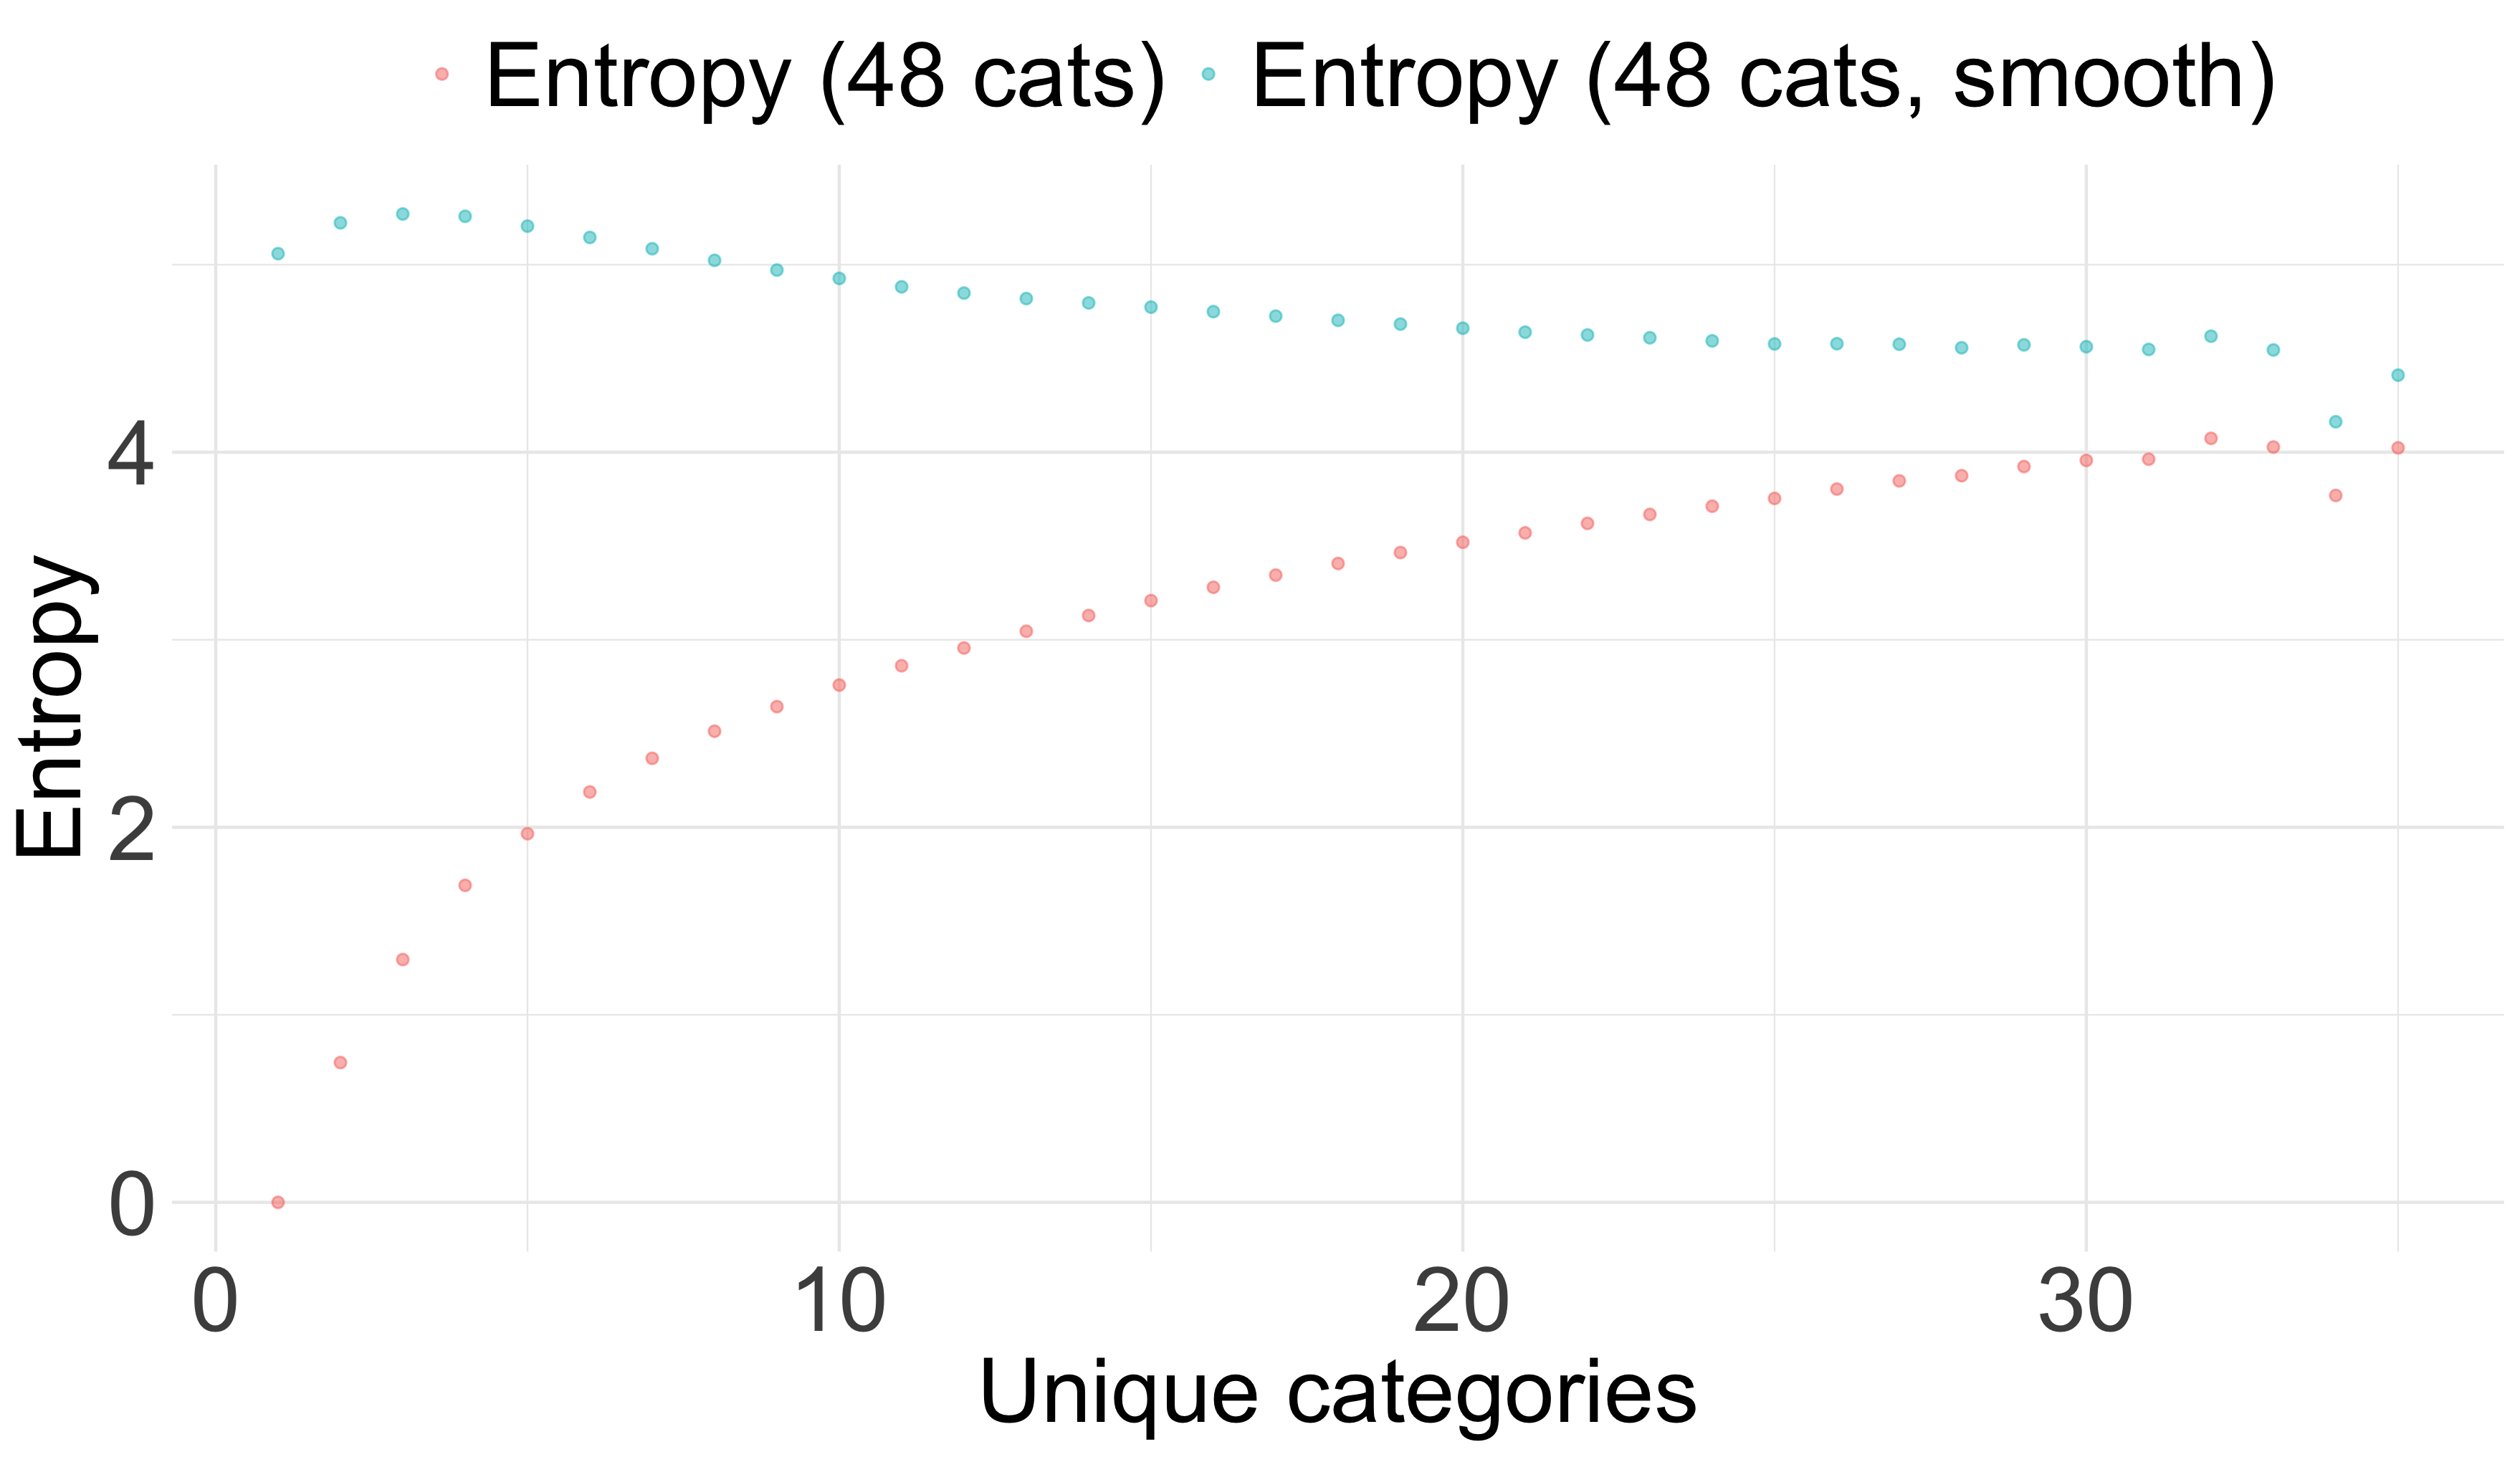
\includegraphics[width=.49\textwidth]{\figdir/smoothing_on_nunique_tag_spend.png}
    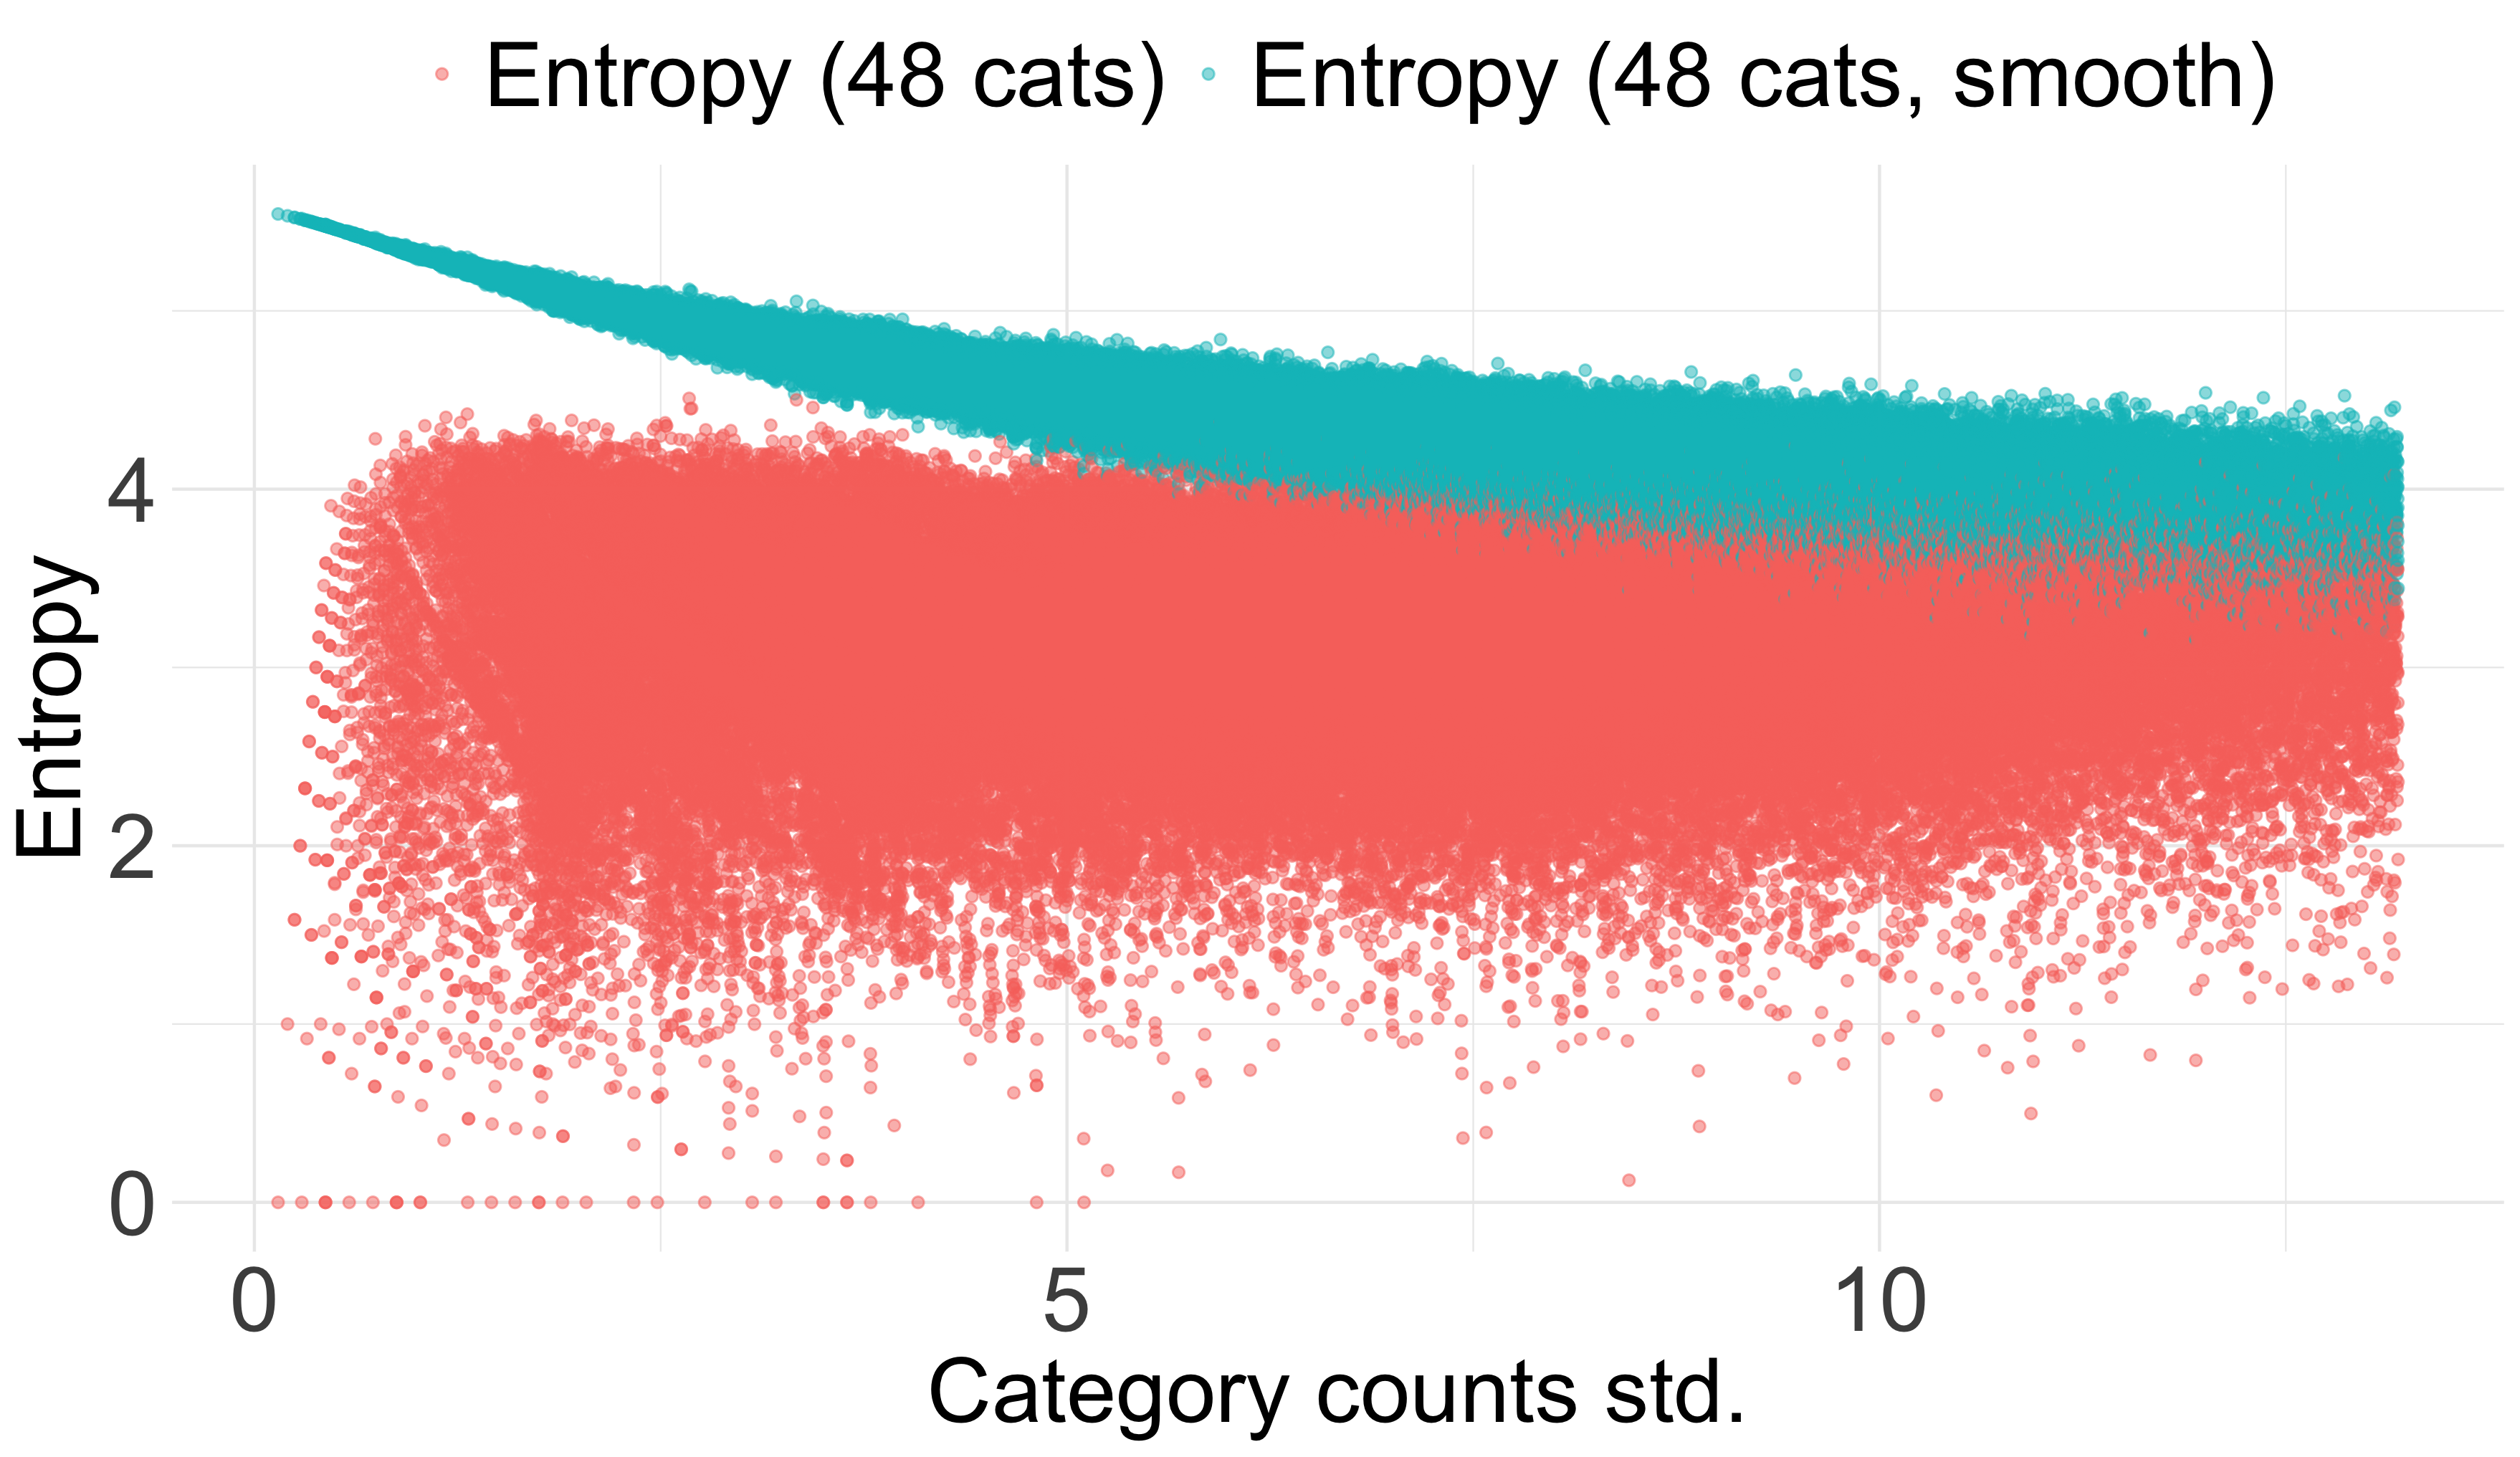
\includegraphics[width=.49\textwidth]{\figdir/smoothing_on_std_tag_spend.png}
    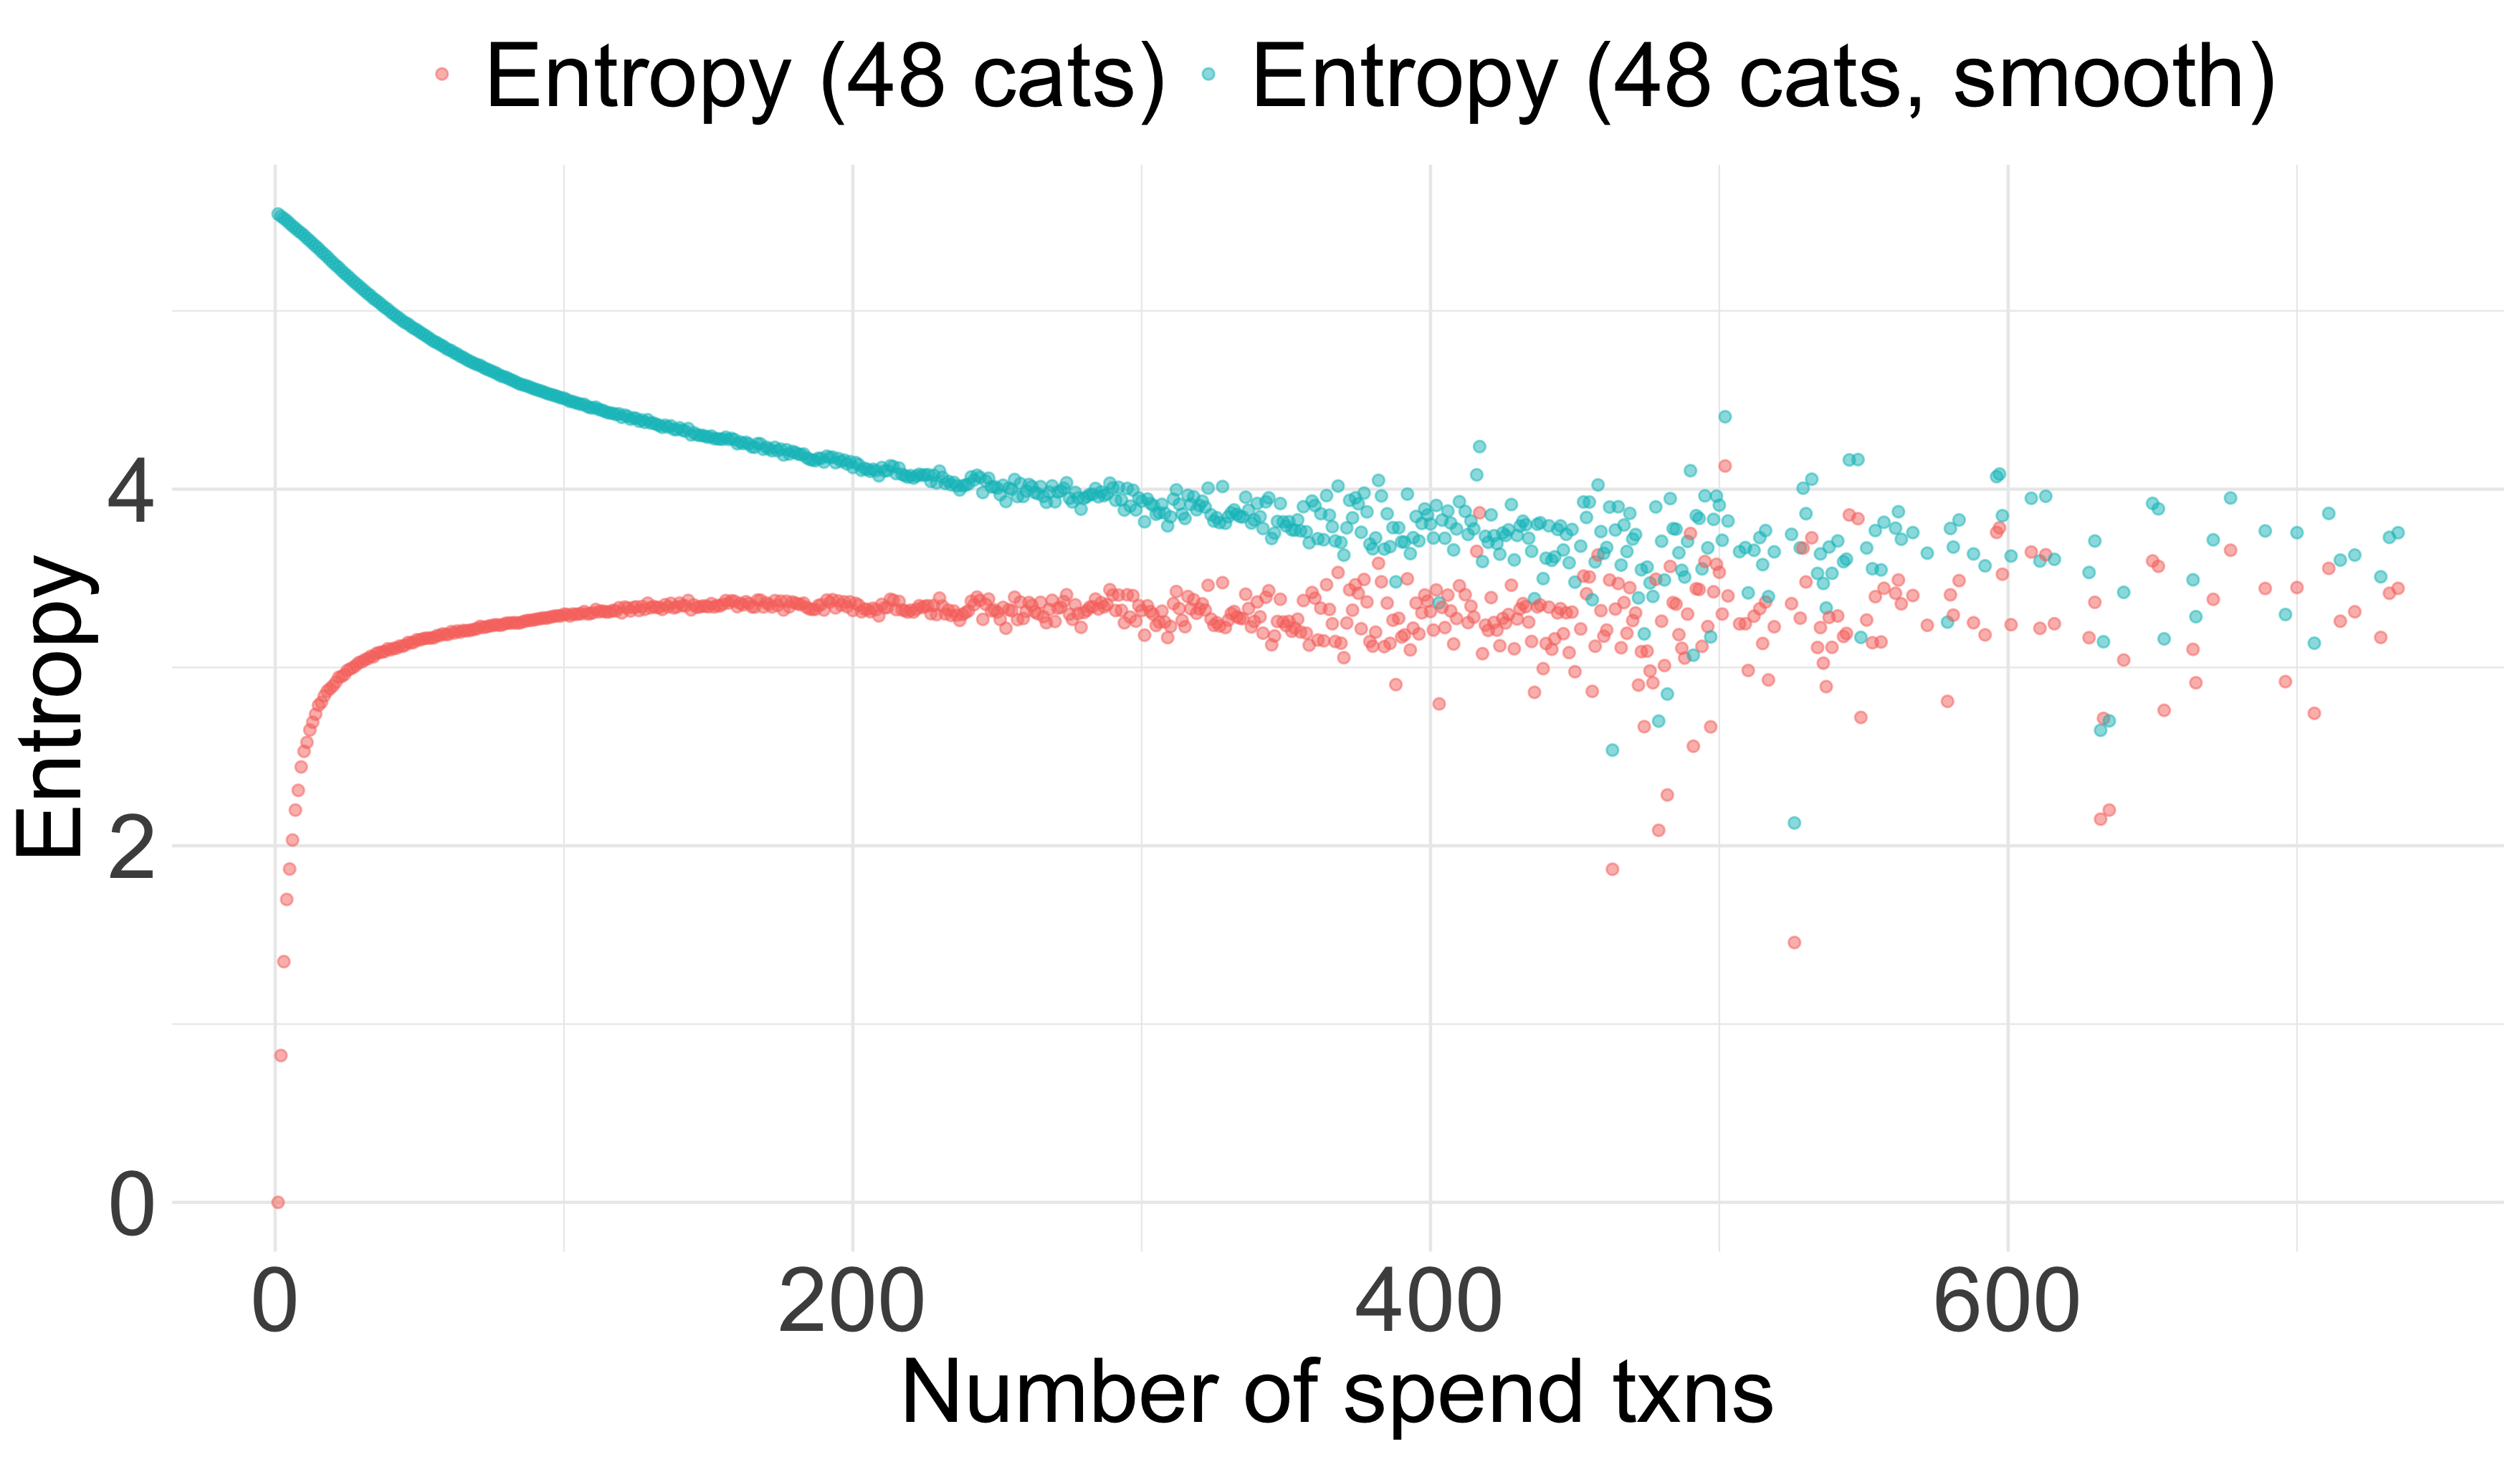
\includegraphics[width=.49\textwidth]{\figdir/smoothing_on_txns_count_spend.png}
    \fignote{\textwidth}{Effect of smoothing on entropy as a function of its
    three main components: the number of spending categories with positive
frequency-counts (left), the standard deviatioin of these counts (middle), and
the total number of spending transaction (right). Value ranges for entropy
components are trimmed at the 95th percentile.}
\end{figure}

- Sign reversal is mechanical
- Interpret in light of formulas
- Suggests that results very fragile to how we define entropy
- Also suggests that sign-issue is a red herring

